\begin{problem}{/images/problems/65_pic.png}{Tiling the $10 \times 10$ Grid} We have a  $10 \times 10$ grid and we want to place a number of $1 \times 5$ and $5 \times 1$ tiles on it so that no two tiles overlap.
	
	What is the minimum number of tiles that can be placed so that there is no room for another tile?
\end{problem}
\begin{solution}
The answer to the problem is 11. An example of a tiling with 11 tiles is shown in the figure below.

\begin{center}
	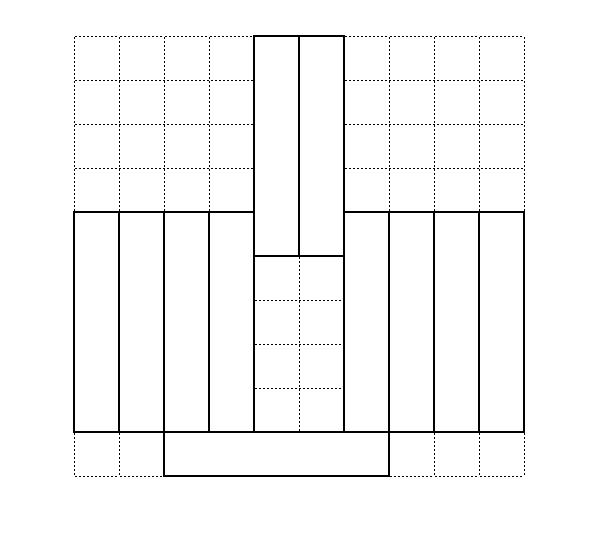
\includegraphics[width=10cm]{/images/problems/65_sol.png}
\end{center}

In general, for tiling a $2n  \times  2n$ grid with vertical or horizontal tiles of length $n$, the answer is $2n + 1$. This can be obtained by generalizing the above tiling schema.

Next, we will discuss why it is not possible to do this with $2n$ tiles. 

\begin{theorem} Theorem 1. If a tiling can be done with $2n$ tiles, then there must be at least one horizontal tile and at least one vertical tile.
\end{theorem}

\begin{proof}We will prove this by contradiction. Suppose all $2n$ tiles are vertical. Then each column must contain at least one tile, otherwise, another tile could be added to that column. On the other hand, the tile in any column cannot start from row 1, because then another tile could be added below that tile in the same column. Therefore, row 1 is empty. Therefore, another horizontal tile could be added in row 1, and the tiling with $2n$ vertical tiles contradicts the problem statement. So our assumption was wrong, and all $2n$ tiles cannot be vertical.

Similarly, it can be proven that not all $2n$ tiles can be horizontal.
\end{proof}

Therefore, there must be at least one vertical tile and at least one horizontal tile in such a solution.

\begin{theorem} Theorem 2. If column $i  \leq n$ contains a vertical tile, then all columns $1$ to $i-1$ also contain vertical tiles.
\end{theorem}
\begin{proof}
	Consider the rectangle between the vertical tile and the left edge of the grid (like the green rectangle in the figure below). Since the width of this rectangle is less than $n$, it cannot contain any horizontal tiles. Therefore, if one of the columns 1 to $i-1$ is empty, then one of the columns in the green section must also be empty, which contradicts the problem statement (no room for another tile).
	
\begin{center}
	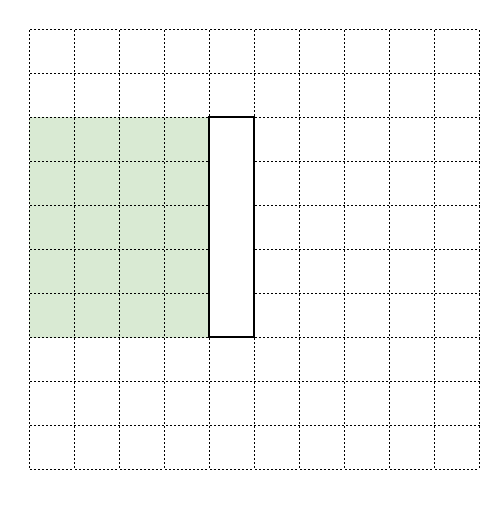
\includegraphics[width=10cm]{/images/problems/65_sol1.png}
\end{center}
	
\end{proof}

Consequences of Theorem 2:

if column $i > n$ contains a vertical tile, then all columns $n+1$ to $2n$ also contain vertical tiles.
Similarly, Theorem 2 and Theorem 1 also hold for rows.

\begin{theorem} Theorem 3. It is not possible to satisfy the problem statement with $2n$ tiles.
\end{theorem}
\begin{proof}
Suppose we have a tiling with at most $2n$ tiles that does not leave room for another tile. Then the minimum number of either horizontal or vertical tiles is at most $n$. Suppose there are at most $n$ vertical tiles.

In this case, according to Theorem 2, all these vertical tiles are placed in a number of consecutive initial columns and a number of consecutive final columns, and at least $n$ consecutive columns in the middle are not blocked by any vertical tile.

According to Theorem 1, the number of vertical tiles is also at least 1, and since we assumed the total number of tiles is at most $2n$, the number of horizontal tiles is at most $2n - 1$. As in the previous point, this means that at least one row in the middle of the grid is not blocked by any horizontal tile.

According to the above points, we conclude that there must be room for another horizontal tile in this arrangement, so the initial assumption was wrong, and it is not possible to satisfy the problem statement with at most $2n$ tiles.
\end{proof}

\end{solution}

